\section{Introdução}\label{sec:introducao}

% - Qual é a da coisa? (sintese c webaudio)
% - como a coisa funciona? 
%   - como um ou outro fez funcionar
%   - nosso jeito de funcionar

% -----------------------------------------------
 % http://www.charlie-roberts.com/pubs/Gibber_charles_roberts_icmc_2012.pdf


A síntese sonora em \emph{web browsers} é sumarizada por \cite{w3c_web_2012,roberts_web_2013-,wyse_viability_2014}. \cite{srikumar_tamming_2013} exemplifica uma concatenação de \emph{nós de áudio} em um grafo de DSP. Três instâncias diferentes, \emph{OscilatorNode}, \emph{GainNode}, \emph{DestinationNode}, são apresentadas na figura \label{fig:chime}. Existe um outro nó, \emph{ScriptProcessorNode} (figura \ref{fig:scriptprocessor}) que possibilita customizações. Por exemplo, pode ser usado para externalizar para um(a) improvisador(a) suas próprias customizações de \emph{funções de transferência} \cite{mathews_groove_1970}. Esta abordagem foi utilizada no desenvolvimento do \emph{Termpot}.

\begin{figure}[!h]
\centering
\caption{Estrutura básica de um sintetizador webaudio. \textbf{Fonte}: \cite{srikumar_tamming_2013}}
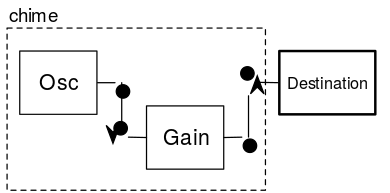
\includegraphics[scale=0.3]{chime.png}
\label{fig:chime}  
\end{figure}


\begin{figure}[!h]
\centering
\caption{``A interface do \emph{ScriptProcessorNode} permite a geração, processamento ou análise de áudio usando JavaScript''. \textbf{Fonte}: \cite{w3c_web_2012}}
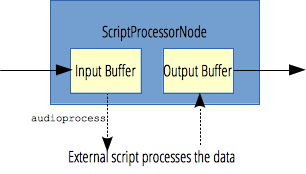
\includegraphics[scale=0.6]{WebAudioScriptProcessingNode.png}
\label{fig:scriptprocessor} 
\end{figure}


\section{Trabalho relacionado: GROOVE}

Este artigo também  envolve uma interpretação do GROOVE, \emph{Generated Real-time Operations On Voltage-controlled Equipment}, de \cite{mathews_groove_1970}. A compositora Laurie Spiegel (figura \ref{fig:groove}) sumariza características, durante a produção de \emph{The Expanding Universe} (1975) \footnote{Disponível em \url{https://www.youtube.com/watch?v=dYUZmsfm4Ww}.}:

\begin{quote}
\small{Todas as músicas no GROOVE eram representadas na memória digital como funções abstratas do tempo, séries paralelas de dois pontos, cada ponto sendo um instante no tempo e um valor instantâneo. A taxa de amostragem para essas funções, usada principalmente como controle de voltagem, era cronometrada por um grande e antiquado oscilador analógico que era normalmente fixado em 100 Hertz, cada ciclo do oscilador pulsando à frente do código, o computador lia, em cada uma das funções, naquele ponto do tempo, todos dispositivos de entrada e executava todas amostras.} \footnote{Tradução de \emph{All music in GROOVE was represented in digital memory as abstract functions of time, parallel series of point pairs, each point being an instant in time and an instantaneous value. The sampling rate for these functions, which would be used mostly as control voltages, was clocked by a big old-fashioned analog oscillator that was usually set to 100 Hertz, each cycle of the oscillator pulsing one run through the code, the computer reading all of the real time input devices and playing of all of the samples at that time point in each of the time functions.}}
\end{quote}

\begin{figure}[!h]
  \begin{center}
  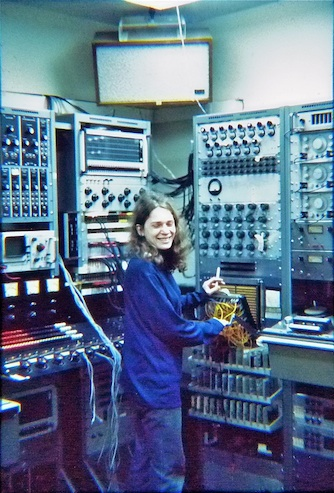
\includegraphics[scale=0.5]{./spiegel.jpg}
  \caption{\small Laurie Spiegel configurando a saída analógica do GROOVE, durante a produção de \emph{The Expanding Universe}. \textbf{Fonte}: \cite{spiegel_expanding_1975}.}
  \label{fig:groove}
  \end{center}
\end{figure}

\section{Objetivo}

\normalsize Sumarizar um programa estruturado no \emph{ScriptProcessorNode} segundo uma interpretação do GROOVE.

%A Seção \ref{sec:trabalhos} deste artigo apresenta os frameworks supracitados e uma breve comparação entre eles.
%A Seção \ref{sec:termpot} apresenta a ferramenta proposta.
%A Seção \ref{sec:resultados} traz os resultados desta pesquisa e a Seção \ref{sec:conclusao} apresenta as conclusões do trabalho até o presente momento.

\section{Metodologia de desenvolvimento}

\begin{inparaenum}[\itshape 1)\upshape]
\item Customização um emulador terminal \emph{Ptty.js} (\footnotesize \url{http://code.patxipierce.com/jquery-plugin/ptty/} \normalsize).
\item Definição de um ambiente interno, baseado no ambiente \emph{Wavepot} (Código-fonte disponível em \footnotesize \url{https://www.github.com/wavepot/wavep0t} \normalsize).
\item Definição de comandos deste ambiente interno: inspeção de funções, definição de novas funções, tocar, parar, pausar, gravar e download, criação de controles gráficos (\emph{jQueryUI}) e gravação (\footnotesize \url{https://github.com/mattdiamond/Recorderjs/blob/master/recorderWorker.js} \normalsize).
\end{inparaenum}

